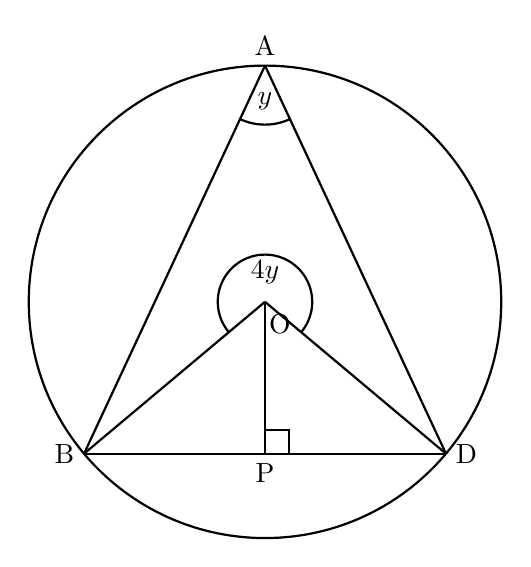
\begin{tikzpicture}[scale=1.5]

    % --- Define Coordinates ---
    % Center O at origin
    \coordinate (O) at (0,0);
    % Radius of the circle
    \def\R{2.0}
    
    % Point A at the top (90 degrees)
    \coordinate (A) at (0, \R);
    
    % Points B and D on the circle
    % Visually, they are symmetric. B around 220 degrees, D around 320 degrees.
    \coordinate (B) at (220:\R);
    \coordinate (D) at (320:\R);
    
    % Point P is the intersection of the vertical line from O and chord BD
    % Since B and D are symmetric about the y-axis, P is on the y-axis
    % P has x=0, y = R * sin(320)
    \coordinate (P) at (0, -1.285); % Approximate y value derived from sin(320)*2

    % --- Draw Circle ---
    \draw[thick] (O) circle (\R);

    % --- Draw Lines and Segments ---
    % Triangle ABD inscribed in the circle
    \draw[thick] (A) -- (B);
    \draw[thick] (A) -- (D);
    \draw[thick] (B) -- (D);

    % Central segments
    \draw[thick] (O) -- (B);
    \draw[thick] (O) -- (D);
    
    % Perpendicular segment OP
    \draw[thick] (O) -- (P);

    % --- Right Angle Symbol at P ---
    % Symbol drawn in the quadrant between OP (up) and PD (right)
    \draw[thick] (0, -1.085) -- (0.2, -1.085) -- (0.2, -1.285);

    % --- Angle Arcs and Labels ---

    % Angle at A (labeled 'y')
    % Vector AB is approx 244 degrees, Vector AD is approx 296 degrees
    \draw[thick] (A) + (244:0.5cm) arc (244:296:0.5cm);
    \node at (0, 1.7) {$y$};

    % Angle at O (labeled '4y')
    % This is the reflex angle (or large upper angle) between OB and OD
    % Arc starts at OD (320 deg) and goes counter-clockwise to OB (220 deg + 360)
    \draw[thick] (O) + (320:0.4cm) arc (320:580:0.4cm);
    \node at (0, 0.25) {$4y$};

    % --- Point Labels ---
    \node[above] at (A) {A};
    \node[left] at (B) {B};
    \node[right] at (D) {D};
    \node[below] at (P) {P};
    % O is placed slightly below-right of the center point in the image
    \node[below right, xshift=-2pt, yshift=-1pt] at (O) {O};

\end{tikzpicture}